\section{ZenML}
\subsection{Installatie}
De installatie van ZenML is via de package manager \texttt{pip} en kan met het volgende commando geïnstalleerd worden.
\begin{minted}[frame=lines,breaklines,linenos]{bash}
    pip install zenml
\end{minted}
Er moet wel rekening gehouden worden dat ZenML alleen werk met de Python versies 3.8, 3.9, 3.10 en 3.11.
Voor het lokaal uitvoeren van het ZenML dashboard moet er ook nog een extra package geïnstalleerd worden:
\begin{minted}[frame=lines,breaklines,linenos]{bash}
    pip install "zenml[server]"
\end{minted}

Nu dat de server geïnstalleerd is kan deze worden opgestart met het volgende commando: 
\begin{minted}{bash}
    zenml up --blocking
\end{minted}
Er wordt een extra parameter \texttt{blocking} toegevoegd omdat Windows ZenML niet als achtergrondproces kan uitvoeren. Het is ook mogelijk om ZenML in een Docker-container uit te voeren met de parameter \texttt{docker}.

Na het opstarten van de server kan in de console het serveradres gevonden worden, zoals te zien is in de figuur~\ref{ZenMLServer}
\begin{figure}
    \centering
    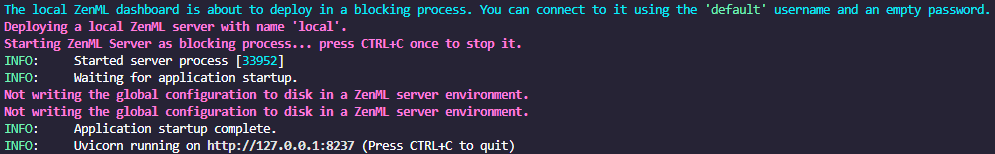
\includegraphics[width=0.9\linewidth]{graphics/ZenML_Server.PNG}
    \caption{ZenML server uitvoer na het opstarten}
    \label{fig:ZenMLServer}
\end{figure}
\subsection{Dashboard}

\subsection{Uitvoering}
\subsection{Pipeline}
\subsection{Problemen}
\subsection{Cloud}
